% !Mode:: "TeX:UTF-8"
\chapter{Nonlinear Optimization}
\label{cpt:6}
\begin{mdframed}  
	\textbf{Goal of This Chapter}
	\begin{enumerate}[labelindent=0em,leftmargin=1.5em]
		\item Understand how to form the batch state estimation problem into a least square and how to solve the least square problem.
		\item Understand the Gauss-Newton and Levenburg-Marquadt method and implement them.
		\item Learn how to use the Google Ceres and g2o library to solve a least square problem.
	\end{enumerate}
\end{mdframed} 

In the previous lectures, we introduced the motion and observation equations of the classic SLAM model. Now we know that the pose in the equation can be described by the transformation matrix and then optimized by Lie algebra. The observation equation is given by the camera imaging model, in which the internal parameter is fixed with the camera, and the external parameter is the pose of the camera. So, we have figured out the concrete expression of the classic visual SLAM model.

However, due to the presence of noise, the equations of motion and observation can not be exactly met. Although the camera can fit the pinhole model very well, unfortunately, the data we get is usually affected by various unknown noises. Even if we have a high-precision camera and controller, the motion and observations equations can only be approximated. Therefore, instead of assuming that the data must conform to the equation, it is better to estimate the state from the noisy data accurately.

Solving the state estimation problem requires a certain degree of optimization background knowledge. This section will introduce the basic unconstrained nonlinear optimization method and introduce optimization libraries g2o and Ceres.

\newpage
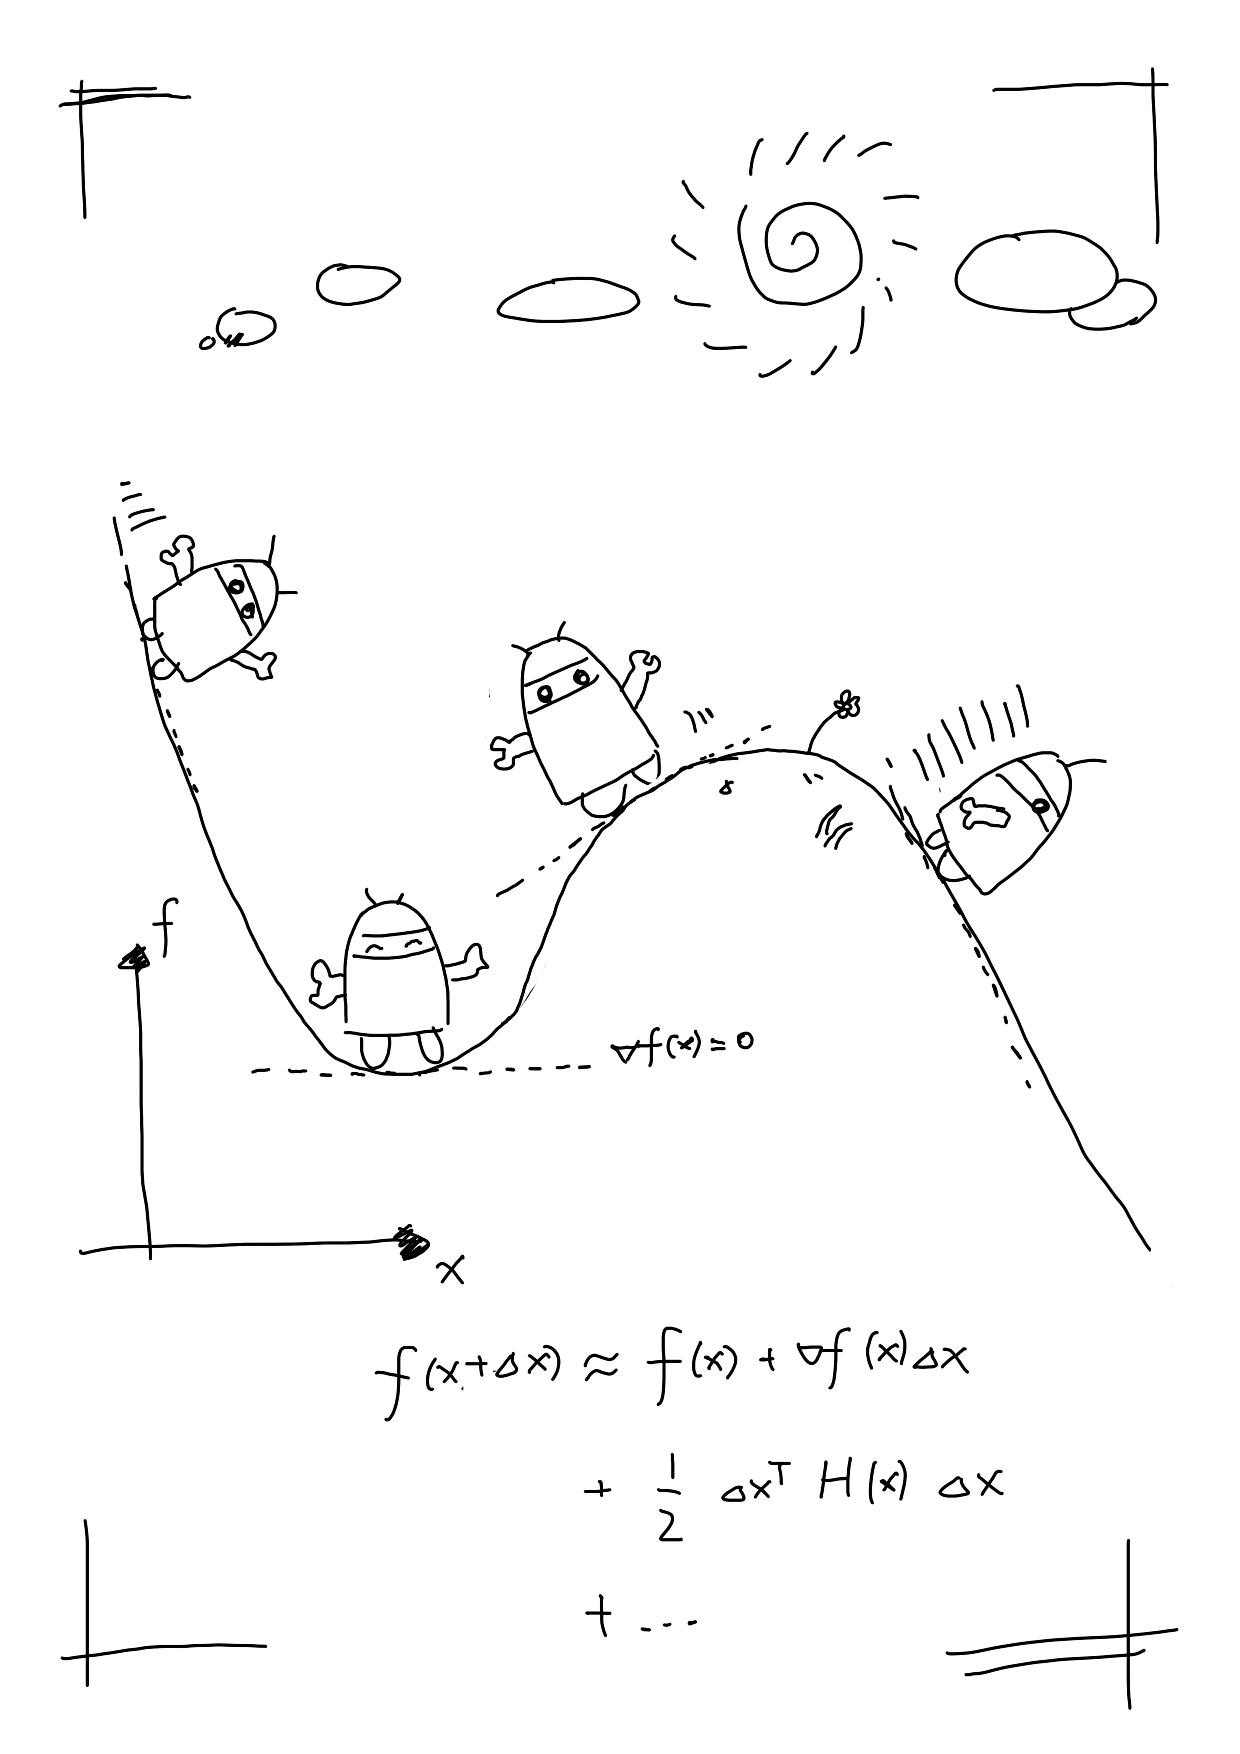
\includepdf{resources/other/ch6.pdf}

\newpage
\section{State Estimation}
\subsection{From Batch State Estimation to Least Square}
According to the previous sections, the SLAM process can be described by a discrete time motion and observation equations like~\eqref{eq:slamproblem}:
\begin{equation}
\left\{ \begin{array}{l}
{\bm{x}_k} = \mathbf{f}\left( {{\bm{x}_{k - 1}},{\bm{u}_k}} \right) + \bm{w}_k\\
{\bm{z}_{k,j}} = \mathbf{h}\left( {{ \bm{y}_j},{ \bm{x}_k}}  \right)+ \bm{v}_{k,j}
\end{array} \right. .
\end{equation}

Through the knowledge in Lecture 4, we learned that $ \bm {x} _k $ is the pose of the camera, which can be described by $ \mathrm {SE} (3) $. As for the observation equation, we have already explained in Lecture 5, the pinhole camera model. In order to give readers a deeper impression of them, we may wish to discuss their specific parameterized form. First, the pose variable $\bm {x} _k $ can be expressed by $\bm {T} _k \in \mathrm {SE} (3) $. Second, the motion is related to the specific form of the input, but there is no particularity in visual SLAM (should be same as the case of ordinary robots and vehicles), we will not talk about it for the time being. The observation equation is given by the pinhole model. Assuming an observation of the road sign $ \bm {y} _j $ at $ \bm {x} _k $, corresponding to the pixel position on the image $ \bm {z} _ {k, j} $, then, observe The equation can be expressed as:
\begin{equation}
s \bm{z}_{k,j}= \bm{K} (\bm{R}_k {\bm{y}_j}+\bm{t}_k),
\end{equation}
where $ \bm {K} $ is the intrinsic matrix of the camera, and $s$ is the distance of pixels, which is also the third element of $ (\bm {R} _k {\bm {y} _j} + \bm {t} _k) $. If we use  transformation matrix $ \bm {T} _k $ to describe the pose, then the points $ \bm {y} _j $ must be described in homogeneous coordinates, and then converted to non-homogeneous coordinates afterwards. If you are not familiar with this process, please go back to the previous lectures.

Now, consider what happens when the data is affected by noise. In the motion and observation equations, we \textbf {usually} assume that the two noise terms $ \bm {w} _k, \bm {v} _ {k, j} $ satisfy a Gaussian distribution with zero mean, like this:
\begin{equation}
{\bm{w}_k} \sim \mathcal{N}\left( {\bm{0},{\bm{R}_k}} \right),{\bm{v}_k} \sim \mathcal{N}\left( {\bm{0},{{{\bm{Q}}}_{k,j}}} \right),
\end{equation}
where $ \mathcal {N} $ means Gaussian distribution, $ \bm{0} $ means zero mean, and $ \bm {R} _k, \bm {Q} _ {k, j} $ is the covariance matrix. Under the influence of these noises, we hope to infer the pose $ \bm {x} $ and the map $ \bm {y} $ from the noisy data $ \bm {z} $ and $ \bm {u} $ (and their probability density distribution), which constitutes a state estimation problem.

There are two ways to deal with this state estimation problem. Since these data come gradually over time in the SLAM process, we should intuitively hold an estimated state at the current moment and then update it with new data. This method is called the \textbf {incremental} method, or \textbf{filtering}. For a long time in history, researchers have used filters, especially the extended Kalman filter (EKF) and its derivatives, to solve it. The other way is to record the data into a file and looking for the best trajectory and map overall time. This method is called the \textbf {batch} estimation. In other words, we can put all the input and observation data from time 0 to $ k $ together and ask, with such input and observation, how to estimate the entire trajectory and map from time 0 to $ k $?

These two different processing methods lead to many estimation methods. In general, the incremental method only cares about the state estimation of the \textbf {current moment} $ \bm {x} _k $, but does not consider much about the previous state; relatively, the batch method can be used to get an optimized trajectory in larger time or space scope, which is considered to be superior to the traditional filters \textsuperscript {\cite {Strasdat2012}}, and has become the mainstream method of current visual SLAM. In extreme cases, we can let robots or drones collect data and then bring it back to the computing center for unified processing, which is also the mainstream practice of SfM (Structure from Motion). Of course, in these cases, the method is obviously not \textbf {real time}, which is not the most common application scenario of SLAM. So in SLAM, practical methods are usually some compromises. For example, we fix some historical trajectories and only optimize some trajectories close to the current moment, which leads to the \textbf {sliding window estimation} method to be described later.

In theory, the batch method is easier to introduce. At the same time, understanding the batch method also makes it easier to understand the incremental method. Therefore, in this section, we focus on the batch optimization method based on nonlinear optimization, and the Kalman filter and more in-depth knowledge will be discussed in the back-end chapter. Since the batch method is discussed, we will consider all the moments from time 1 to $N$ and assume $M$ map points. Define the robot pose and map coordinates at all times as:
\[
\bm{x}=\{ \bm{x}_1, \ldots, \bm{x}_N \}, \quad \bm{y} = \{\bm{y}_1, \ldots, \bm{y}_M \}.
\]
Similarly, $ \bm {u} $ without subscript is used for input at all times, and $ \bm {z} $ is used for observation data at all times. Then we say that the state estimation of the robot, from a probabilistic point of view, is to find the state $ \bm {x}, \bm{y}$ under the condition that the input data $ \bm {u} $ and the observation data $\bm{z} $. Or, the conditional probability distribution of:
\begin{equation}
P( \bm{x},\bm{y} | \bm{z}, \bm{u}).
\end{equation}

In particular, when we do not know the control input and only have one image, that is, only considering the data brought by the observation equation, it is equivalent to estimate  the conditional probability distribution $ P (\bm {x}, \bm {y} | \bm { z}) $. Such a problem is also called Structure from Motion (SfM), that is, how to reconstruct the three-dimensional spatial structure from images only \textsuperscript {\cite {Agarwal2009}}.

To estimation the conditional pdf we use the Bayes equation to switch the variables:
\begin{equation}
P\left( { \bm{x},\bm{y}| \bm{z}, \bm{u}} \right) = \frac{{P\left( {\bm{z},\bm{u}|\bm{x},\bm{y}} \right)P\left( \bm{x}, \bm{y} \right)}}{{P\left( \bm{z},\bm{u}\right)}} \propto \underbrace{P\left(  { \bm{z},\bm{u}| \bm{x},\bm{y} } \right)}_{\text{likehood}} \underbrace{P\left( \bm{x},\bm{y} \right)}_{\text{prior}}.
\end{equation}

The left side is called \textbf {posterior probability}, and $ P (\bm {z} | \bm {x}) $ on the right is called \textbf {likelihood} (or likehood), and the other part is $ P (\bm {x}) $ is called \textbf {prior}. \textbf {It is normally difficult to find the posterior distribution directly (in nonlinear systems), but it is feasible to find an optimal point which maximize the posterior} (Maximize a Posterior, MAP):
\begin{equation}
{(\bm{x},\bm{y})^*}_{\mathrm{MAP}} = \arg {\mathop{\rm max}\nolimits} P \left( {\bm{x},\bm{y}|\bm{z},\bm{u}} \right) = \arg \max P(\bm{z},\bm{u}|\bm{x},\bm{y})P(\bm{x},\bm{y}).
\end{equation}

Please note that the denominator part of Bayes' rule has nothing to do with the state $ \bm {x}, \bm {y} $ to be estimated, so it can be just ignored. Bayes' rule tells us that solving the maximum posterior probability is \textbf {equivalent to the estimate the product of maximum likelihood and a priori}. Further, we can also say ``I'm sorry, I don't know in prior where the robot pose or the map points are'', then there is no \textbf {prior}. Then, you can solve \textbf {Maximize Likelihood Estimation} (MLE):
\begin{equation}
{ (\bm{x},\bm{y})^*}_{\mathrm{MLE}} = \arg \max P( \bm{z},\bm{u}| \bm{x},\bm{y}).
\end{equation}

Intuitively speaking, likelihood refers to ``what observation data may be generated in the current pose''. Since we know the observation data, the maximum likelihood estimation can be understood as: ``\textbf{under what state is it most likely to produce the data currently observed}''. 

\subsection{Introduction to Least Squares}
Now we have a formulated the state estimation problem into a MAP/MLE problem, and the next question is how to solve it. Under the assumption of Gaussian distribution, we can have a simpler form of the maximum likelihood problem. Looking back at the observation model, for a certain kind of observation, we have:
\[
{\bm{z}_{k,j}} = h\left( {{ \bm{y}_j},{ \bm{x}_k}} \right)+ \bm{v}_{k, j},
\]
Since we assume the noise item is gaussian, which means ${\bm{v}_k} \sim \mathcal{N}\left( {\bm{0},{{{\bm{Q}}}_{k,j}}} \right)$, so the conditional probability of the observation data is:
\[
P( \bm{z}_{j,k} | \bm{x}_k, \bm{y}_j) = N\left( h(\bm{y}_j, \bm{x}_k), \bm{Q}_{k,j} \right),
\]
which is, of course, still a Gaussian distribution. Now let's consider solving the maximum likelihood estimation under this single observation.

We can rewrite this maximum problem into a \textbf{minimium of negative logarithm} one for Gaussian distributions since they have better mathematical forms under negative logarithm. Consider an arbitrary multi-dimensional Gaussian distribution $\bm{x} \sim \mathcal{N}(\bm{\mu}, \bm{\Sigma})$, its probability density function expansion form is:
\begin{equation}
	P\left( \bm{x} \right) = \frac{1}{{\sqrt {{{(2\pi )}^N}\det (\bm{\Sigma} )} }}\exp \left( {-\frac{1}{2}{{\left( {\bm{x}-\bm{\mu}} \right)}^\mathrm{T}}{ \bm{\Sigma} ^ {-1}}\left( {\bm{x}-\bm{\mu}} \right)} \right).
\end{equation}
Taking the negative logarithm of both sides:
\begin{equation}
	-\ln \left( {P\left( \bm{x} \right)} \right) = \frac{1}{2}\ln \left( {{{\left( {2\pi} \right )}^N}\det \left( \bm{\Sigma} \right)} \right) + \frac{1}{2}{\left( {\bm{x}-\bm{\mu}} \right)^\mathrm{T}}{\bm{\Sigma} ^{-1}}\left( {\bm{x}-\bm{\mu}} \right).
\end{equation}
Because the logarithm function is monotonically increasing, maximizing the original function is equivalent to minimizing the negative logarithm. When minimizing $\bm{x}$ in the above formula, the first term has nothing to do with $\bm{x}$ and can be omitted. Therefore, as long as the quadratic term on the right is minimized, the maximum likelihood estimate of the state is obtained. Substituting into the SLAM observation model, it is equivalent to find such a solution:
\begin{equation}
	\begin{aligned}
		(\bm{x}_k,\bm{y}_j)^* &= \arg \max \mathcal{N}(h(\bm{y}_j, \bm{x}_k), \bm{Q }_{k,j}) \\ &= \arg \min \left( {{{\left( {{ \bm{z}_{k,j}}-h\left( {{\bm{x }_k},{\bm{y}_j}} \right)} \right)}^\mathrm{T}} \bm{Q}_{k,j}^{-1}\left( {{\ bm{z}_{k,j}}-h\left( {{\bm{x}_k},{\bm{y}_j}} \right)} \right)} \right).
	\end{aligned}
\end{equation}

We found that this equation is equivalent to a quadratic form that minimizes the noise term (i.e., the error). This quadratic form is called \textbf{Mahalanobis distance}. It can also be regarded as the Euclidean distance ($\mathcal{L}_2$-norm) weighted by $\bm{Q}_{k,j}^{-1}$, where $\bm{Q}_{k,j} ^{-1}$ is also called the \textbf{information matrix}, which is extacly the \textbf{inverse} of the Gaussian  \textbf{covariance matrix}.

Now we put all the observations together. It is usually assumed that the inputs and observations at each time are independent of each other, which means that each input is independent, each observation is independent, and input and observation are also independent. So we can factorize the joint distribution like this:
\begin{equation}
	P\left( {\bm{z},\bm{u}|\bm{x},\bm{y}} \right) = \prod\limits_k {P\left( {{\bm{u}_k }|{\bm{x}_{k-1}},{\bm{x}_k}} \right)} \prod\limits_{k,j} {P\left( {{\bm{z} _{k,j}}|{\bm{x}_k},{\bm{y}_j}} \right)},
\end{equation}

It shows that we can handle the movement and observation at each moment independently. Let's define the error between the model and real data: 
\begin{equation}
	\begin{array}{l}
		{\bm{e}_{u,k}} = {\bm{x}_k}-f\left( {{\bm{x}_{k-1}},{\bm{u}_k} } \right)\\
		{\bm{e}_{z,j,k}} = {\bm{z}_{k,j}}-h\left( {{\bm{x}_k},{\bm{y} _j}} \right),
	\end{array}
\end{equation}
Then, minimizing the Mahalanobis distance between the estimated value at all times and the measurements from sensors is equivalent to finding the maximum likelihood estimation. The negative logarithm allows us to turn the product into a summation:
\begin{equation}
	\label{eq:least-square}
	\min J (\bm{x},\bm{y}) = \sum\limits_k {\bm{e}_{u,k}^\mathrm{T} \bm{R}_k^{-1} {\bm{e}_{u,k}}} + \sum\limits_k {\sum\limits_j {\bm{e}_{z,k,j}^\mathrm{T} \bm{Q}_ {k,j}^{-1}{\bm{e}_{z,k,j}}}}.
\end{equation}
In this way, a \textbf{least square problem} is obtained with the same solution as the MLE problem. Intuitively speaking, due to the presence of noise, when we substitute the estimated trajectory and map into the SLAM motion and observation models, they will not be perfectly fit. What shall we do at this time? We perform \textbf{fine-tuning} on the estimated value of the state, so that the overall error is reduced. Of course, finally we will reach a (local) \textbf{minimum value}. This is a typical nonlinear optimization process.

Observing the formula~\eqref{eq:least-square} carefully, we find that the least squares problem in SLAM has some specific structures:

\begin{itemize}
	\item First, the objective function of the whole problem consists of many (weighted) error quadratic forms. Although the dimensionality of the overall state variable is very high, each error term is simple and is only related to one or two state variables. For example, the motion error is only related to $\bm{x}_{k-1}, \bm{x}_k$, and the observation error is only related to $\bm{x}_k, \bm{y}_j$. This relationship will give a \textbf{sparse} least square problem, which we will investigate further in the backend chapter.

	\item Secondly, if you use Lie algebra to represent the increment, the problem is the least squares problem of \textbf{unconstrained}. However, if the rotation matrix/transformation matrix is ​​used to describe the pose, the constraint of the rotation matrix itself will be introduced, that is, $\mathrm{s.t.}\ \bm{R}^\mathrm{T} \bm{R} = \bm{I}$ and $\det (\bm{R})=1$ need to be added to the problem. Additional constraints can make optimization more difficult.

	\item Finally, we used a quadratic metric error, which is exactly the $\mathcal{L}_2-$norm. The information matrix is used as the weights of each elemnents. For example, if an observation is very accurate, the covariance matrix will be ``small'' and the information matrix will be ``large'', so this error term will have a higher weight than the others in the whole problem. We will see some drawbacks of the $\mathcal{L}_2$ error later.
\end{itemize}

We introduce how to solve this least-squares problem, which requires some \textbf{basic knowledge of nonlinear optimization}. In particular, we want to discuss how to solve such a general unconstrained nonlinear least-squares problem. In the following lectures, we will make extensive use of this lecture's results and discuss in detail its application in the front and back ends of SLAM\@.

\subsection{Example: Batch state estimation}
Maybe it's better to give an example here. Consider a very simple discrete-time system:
\begin{equation}
    \begin{array}{lll}
        {x_k} &= {x_{k-1}} + {u_k} + {w_k},&\qquad w_k \sim \mathcal{N}\left( {0,Q_k} \right)\\
        {z_k} &= {x_k} + {n_k},&\qquad {n_k}\sim \mathcal{N}\left( {0,R_k} \right)
    \end{array},
\end{equation}
which can express a car moving forward or backward along the $x$ axis. The first formula is the motion model, where $u_k$ is the input, and $w_k$ is the noise; the second formula is the observation model, where $z_k$ is the measurement of the car position. We set the time $k=1,\ldots,3$, and want to estimate the states based on the existing $v,y$. Suppose the initial state $x_0$ is known. Let's derive the maximum likelihood estimation of the batch state estimation.

First, let the batch state variable be $\bm{x} = [x_0,x_1, x_2, x_3]^\mathrm{T}$, and the batch observation be $\bm{z} = [z_1,z_2,z_3]^ \mathrm{T}$, define $\bm{u}=[u_1,u_2,u_3]^\mathrm{T}$ in the same way. According to the previous derivation, we know that the maximum likelihood estimate is:
\begin{equation}
    \begin{aligned}
        {\bm{x}_{\mathrm{map}}^*} &= \arg \max P(\bm{x}|\bm{u},\bm{z}) = \arg \max P( \bm{u},\bm{z}|\bm{x})\\
        &= \prod\limits_{k = 1}^3 {P({u_k}|{x_{k-1}},{x_k})\prod\limits_{k = 1}^3 {P\left( { {z_k}|{x_k}} \right)} },
    \end{aligned}
\end{equation}
For each item, such as the equation of motion, we have:
\begin{equation}
    P({u_k}|{x_{k-1}},{x_k}) = \mathcal{N}({x_k}-{x_{k-1}},{Q_k}).
\end{equation}
The observation equation is similar:
\begin{equation}
    P\left( {{z_k}|{x_k}} \right) = \mathcal{N}\left( {{x_k},{R_k}} \right).
\end{equation}

According to the previous statements, the error variable can be constructed as:
\begin{equation}
    {e_{u,k}} = {x_k}-{x_{k-1}}-{u_k}, \quad {e_{z,k}} = {z_k}-{x_k},
\end{equation}
Then the objective function of the least squares is:
\begin{equation}
    \min \sum\limits_{k = 1}^3 {e_{u,k}^\mathrm{T} Q_k^{-1}{e_{u,k}}} + \sum\limits_{k = 1 }^3 {e_{z,k}^\mathrm{T}{R^{-1}_k}{e_{z,k}}}.
\end{equation}

In addition, since this system is a linear one, we can easily write the equations in the vector/matrix form. Define the vector $\bm{y}=[\bm{u}, \bm{z}]^\mathrm{T}$, then the error can be defined as:
\begin{equation}
    \bm{y}-\bm{H}\bm{x} = \bm{e} \sim \mathcal{N}(\bm{0}, \boldsymbol{\Sigma}),
\end{equation}
where
\begin{equation}
    \bm{H} = \left[ {\begin{array}{*{20}{c}}
            1&{-1}&0&0\\
            0&1&{-1}&0\\
            0&0&1&{-1}\\
            \hline
            0&1&0&0\\
            0&0&1&0\\
            0&0&0&1
    \end{array}} \right],
\end{equation}
and $\boldsymbol{\Sigma}=\mathrm{diag}(Q_1, Q_2, Q_3, R_1, R_2, R_3)$. The whole question can be written as:
\begin{equation}
    \bm{x}^*_{\mathrm{map}} = \arg \min \bm{e}^\mathrm{T} \boldsymbol{\Sigma}^{-1} \bm{e},
\end{equation}
Later we will see that this problem has a unique solution:
\begin{equation}
    \bm{x}^*_{\mathrm{map}} = (\bm{H}^\mathrm{T} \boldsymbol{\Sigma}^{-1} \bm{H})^{-1} \bm{H}^\mathrm{T} \boldsymbol{\Sigma}^{-1} \bm{y},
\end{equation}
since the $(\bm{H}^\mathrm{T} \boldsymbol{\Sigma}^{-1} \bm{H})^{-1}$ is invertible.

\section{Nonlinear least squares}
\label{sec:6.2}
First consider a simple least squares problem:
\begin{equation}
    \mathop {\min }\limits_{\bm{x}} F(\bm{x}) = \frac{1}{2}{\left\| {f\left( \bm{x} \right) } \right\|^2_2}.
\end{equation}

Among them, the status variable is $\bm{x} \in \mathbb{R}^n$, and $f$ is any scalar nonlinear function $f(\bm{x}): \mathbb{R}^n \mapsto \mathbb{R}$. Note that the coefficient $\frac{1}{2}$ here is not important, some literature have this coefficient and some not. It will not affect the subsequent conclusions. Obviously, if $f$ is a mathematically simple function, then the problem can be solved in analytical form. Let the derivative of the objective function be zero, and then find the optimal value of $\bm{x}$, just like finding the extreme value of a scalar function:
\begin{equation}
    \frac{ \mathrm{d} F}{ \mathrm{d} \bm{x}} = \bm{0}.
\end{equation}

We reach the minimum, maximum, or saddle points by solving this equation (or, intuitively, by letting the derivative be zero). But is this equation easy to solve? Well, it depends on the form of the derivative function of $f$. If $f$ is just a simple linear function, then the problem is only a simple linear least squares problem. Still, some derivative functions may be complicated in form, making the equation difficult to solve. Solving this equation requires us to know the \textbf{global property} of the objective function, which is usually not possible. For the least squares problem that is inconvenient to solve directly, we can use \textbf{iterated methods} to start from an initial value and continuously update the current estimations to reduce the objective function. The specific steps can be listed as follows:

\begin{mdframed}  
    \begin{enumerate}
        \item Give an initial value $\bm{x}_0$.
        \item For $k$-th iteration, we find an incremental value of $\Delta \bm{x}_k$, such that the object function $\left\| {f\left( \bm{x}_k + \Delta \bm{x}_k \right)} \right \|^2_2$ reaches a smaller value.
        \item If $\Delta \bm{x}_k$ is small enough, stop the algorithm.
        \item Otherwise, let $\bm{x}_{k+1} = \bm{x}_k+\Delta \bm{x}_k$ and return to step 2.
    \end{enumerate}
\end{mdframed}

Now things get much simpler. We turn the problem of solving \textbf{the derivative function equals zero} into a problem of \textbf{looking for decreasing increments} $\Delta \bm{x}_k$. We will see that since the objective function can be linearly approximated at the current estimation, the increment calculation will be simpler \footnote{Linear cases are always the easiest ones.}. When the function decreases until the increment becomes very small, it is considered that the algorithm converges, and the objective function reaches a minimum value. In this process, the problem is how to find the increment at each iteration point, which is a local problem. We only need to be concerned about the local properties of $f$ at the iteration value rather than the global properties. Such methods are widely used in optimization, machine learning, and other fields.

Next, we examine how to find this increment $\Delta \bm{x}_k$. This part of knowledge belongs to the field of numerical optimization. Let's take a quick look at some widely used results.

\subsection{First and Second-order Method}
Now consider the $k$-th iteration. Suppose we are at $\bm{x}_k$ and want to find the increment $\Delta \bm{x}_k$, then the most intuitive way is to make the Taylor expansion of the objective function in $\bm{x}_k$:
\begin{equation}
    F(\bm{x}_k+\Delta \bm{x}_k) \approx F{\left( \bm{x}_k \right)} + \bm{J} \left( \bm{x}_k \right) ^\mathrm{T} \Delta \bm{x}_k + \frac{1}{2}\Delta {\bm{x}_k^\mathrm{T}}\bm{H}(\bm{ x}_k) \Delta \bm{x}_k,
\end{equation}
where $\bm{J}(\bm{x}_k)$ is the first derivative of $F(\bm{x})$ with respect to $\bm{x}$ (also called gradient, \textbf{Jacobi} Matrix, or \textbf{Jacobian}) \footnote{We write $\bm{J}(\bm{x})$ as a column vector, then it can be inner product with $\Delta \bm{x}$ to get a scalar. }, $\bm{H}$ is the second-order derivative (or \textbf{Hessian}), which are all taken at $\bm{x}_k$. Readers should be familiar with them in the undergraduate course like multivariate calculus. We can choose to keep the first-order or second-order terms of the Taylor expansion, and the corresponding solution is called the first-order or the second-order method. In the simplest way, if we only keep the first-order one, then taking the increment at the minus gradient direction will ensure that the function decreases: 
\begin{equation}
    \Delta \bm{x}^* =-\bm{J}(\bm{x}_k).
\end{equation}

Of course, this is only a direction, usually we have to compute another step length parameter, say, $\lambda$. The step length can be calculated according to certain conditions \textsuperscript{\cite{Wolfe1969}}. There are also some empirical methods in machine learning, but we will not discuss them. This method is called \textbf{steepest descent method}. Its intuitive meaning is very simple, as long as we move along the reverse gradient direction, the objective function must decrease if the first-order (linear) approximation still holds.

Note that the above discussion was carried out during the $k$-th iteration and did not involve any information about $k$. To simplify the notation, we will omit the subscript $k$ later and think that these discussions are valid for any iterations.

On the other hand, we can choose to keep the second step information, and the increment equation is:
\begin{equation}
    \Delta \bm{x}^* = \arg \min \left(F\left( \bm{x} \right) + \bm{J} \left( \bm{x} \right)^\mathrm{ T} \Delta \bm{x} + \frac{1}{2}\Delta {\bm{x}^\mathrm{T}}\bm{H} \Delta \bm{x} \right).
\end{equation}
The right side only contains the zero-order, first-order and quadratic terms of $\Delta \bm{x}$. Finding the derivative of $\Delta \bm{x}$ on the right side of the equation and setting it to zero leads to: \footnote{For students who are not familiar with matrix derivation, please refer to Appendix B. }
\begin{equation}
    \label{eq:newton-method}
    \bm{J} + \bm{H} \Delta \bm{x} = \bm{0} \Rightarrow
    \bm{H} \Delta \bm{x} = -\bm{J}.
\end{equation}

We can also solve this linear equation and get the increment. This method is also called \textbf{Newton's method}.

We have seen that both the first-order and second-order methods are very intuitive, as long as we can calculate Taylor expansion of $f$ and find the increments. We say, hey, the function looks like a linear or quadratic one. We can use the approximated function's minimum value to guess the minimum value of the original function. As long as the original objective function really looks like a first-order or quadratic function locally, this type of algorithm is always valid (this is also most cases in reality). However, these two methods also have their drawbacks. The steepest descent method is too greedy and easy to lead a zigzag way and increases the number of iterations. However, Newton's method needs to calculate the $\bm{H}$ matrix of the objective function, which is very time-expensive when the problem is large, and we usually tend to avoid the calculation of $\bm{H}$. For general problems, some quasi-Newton methods can get better results, and for least squares problems, there are several more practical methods: the \textbf{Gauss-Newton's method} and the (Levernburg-Marquardt's method).

\subsection{The Gauss-Newton Method}
The Gauss-Newton method is one of the simplest methods in optimization algorithms. Its idea is to carry out a first-order Taylor expansion of $f(\bm{x})$. Please note that this is not the objective function $F(\bm{x})$ but the lower case $f(\bm{x})$, otherwise it is same as the Newton's method.
\begin{equation}
    \label{eq:approximation}
    f\left( {\bm{x} + \Delta \bm{x}} \right) \approx f\left( \bm{x} \right) + \bm{J} \left( \bm{x} \right)^\mathrm{T} \Delta \bm{x}.
\end{equation}

Here $\bm{J}(\bm{x})$ is the derivative of $f(\bm{x})$ with respect to $\bm{x}$, which is a column vector of $n \times 1$. According to the previous framework, the current goal is to find the increment $\Delta \bm{x}$ such that $\left\| {f\left( \bm{x} + \Delta \bm{x} \right)} \right \|^2$ reached the minimum. In order to find $\Delta \bm{x}$, we need to solve a linear least square problem:
\begin{equation}
    \Delta \bm{x}^* = \arg \mathop {\min }\limits_{\Delta \bm{x}} \frac{1}{2}{\left\| {f\left( \bm{x} \right) + \bm{J} \left( \bm{x} \right)^\mathrm{T} \Delta \bm{x} } \right\|^2}.
\end{equation}
    
What's the difference from before? According to the extreme conditions, we set the derivative with $\Delta \bm{x}$ to zero to reach the extreme value. To do this, let's first expand the square term of the objective function:
\begin{align*}
    \frac{1}{2}{\left\| {f\left( \bm{x} \right) + \bm{J} \left( \bm{x} \right)^\mathrm{T} \Delta \bm{x}} \right\|^2} &= \frac{1}{2}{\left( {f\left( \bm{x} \right) + \bm{J}\left( \bm{x} \right)^\mathrm{T} \Delta \bm{x}} \right)^\mathrm{T}}\left( {f\left( \bm{x} \right) + \bm{J} \left( \bm{x} \right)^\mathrm{T} \Delta \bm{x}} \right)\\
    &= \frac{1}{2}\left( \| f{{\left( \bm{x} \right)}\|^2_2 + 2 f\left( \bm{x} \right) \bm{J} {{\left( \bm{x} \right)}}^\mathrm{T} \Delta \bm{x} + \Delta { \bm{x}^\mathrm{T}}{\bm{J} (\bm{x})} \bm{J}(\bm{x})^\mathrm{T} \Delta \bm{x}} \right).
\end{align*}


Find the derivative of the above formula with respect to $\Delta \bm{x}$ and set it to zero:
\begin{displaymath}
    \bm{J} {\left( \bm{x} \right)}f\left( \bm{x} \right) + \bm{J} {\left( \bm{x} \right)} \bm{J}^\mathrm{T} \left( \bm{x} \right)\Delta \bm{x} = \bm{0}.
\end{displaymath}

The following equations can be obtained:
\begin{equation}
    \underbrace{\bm{J} {\left( \bm{x} \right)} \bm{J}^\mathrm{T}}_{\bm{H}(\bm{x})} \left( \bm{x} \right)\Delta \bm{x} =  \underbrace{- \bm{J} {\left( \bm{x} \right)} f\left( \bm{x} \right)}_{\bm{g}(\bm{x})}.
\end{equation}

This equation is a \textbf{linear equation} of the variable $\Delta \bm{x}$. We call it \textbf{normal equation} or \textbf{Gauss-Newton equation}. We define the coefficients on the left as $\bm{H}$ and the coefficient on the right as $\bm{g}$, then the above formula becomes:
\begin{equation}
    \label{eq:minimize-deltax}
    \bm{H} \Delta \bm{x} = \bm{g}.
\end{equation}
It makes sense to mark the left side as $\bm{H}$ here. Compared with Newton's method~\ref{eq:newton-method}, Gauss-Newton's method uses $\bm{J}\bm{J}^\mathrm{T}$ \textbf{as the approximation} of the second-order Hessian matrix in Newton's method, thus omitting the calculation of $\bm{H}$. Please note that solving the normal equation is the core of the entire optimization problem. If we can get the $\Delta \bm{x}$ in each iteration, then the algorithm of Gauss-Newton method can be written as:

\begin{mdframed}
    \begin{enumerate}
        \item Set it initial value as $\bm{x}_0$.
        \item For $k$-th iteration,calculate the Jacobian $\bm{J}(\bm{x}_k)$ and residual $f(\bm{x}_k)$.
        \item Solve the normal equation: $\bm{H} \Delta \bm{x}_k = \bm{g}$.
        \item If $\Delta \bm{x}_k$ is small enough, stop the algorithm. Otherwise let $\bm{x}_{k+1} = \bm{x}_k+\Delta \bm{x}_k$ and return to step 2.
    \end{enumerate}
\end{mdframed}

It can be seen from the algorithm steps that the solution of the incremental equation occupies a major position. As long as we can solve the increment smoothly, we can ensure that the objective function decreases correctly.

In order to solve the incremental equation, we need to solve $\bm{H}^{-1}$, which requires the $\bm{H}$ matrix to be invertible, but the calculated $\bm{J} \bm{ J}^\mathrm{T}$ is only semi-positive definite. If $\bm{J}$ has null-spaces, which is to say, we can find non-zero $\Delta \bm{x}$ such that $\bm{J} \Delta\bm{x} = \bm{0}$, then we can not determine which $\Delta \bm{x}$ can really makes the objective function really decreases. In that cases, the algorithm is probably not converging and we may obtain erroneous results. Intuitively, the local approximation of the original function at this point is not like a quadratic function. Furthermore, even if we assume that $\bm{H}$ is not singular or ill-conditioned, but if we take a very large step size $\Delta \bm{x}$, the result can still be bad since linear approximation is not accurate enough at that point. So in practice, we can't guarantee that the Gauss-Newton method converges. Sometimes they can reach even larger objective functions values that the initial one. 

Although the Gauss-Newton method has these shortcomings, it is still a simple and effective method for nonlinear optimization, and it is worth learning. In nonlinear optimization, quite a few algorithms can be taken as the variants of the Gauss-Newton method. These algorithms all use the idea of the Gauss-Newton method and correct their shortcomings through their own improvements. For example, some \textbf{line search method} adds an extra step size $\alpha$. After determining $\Delta \bm{x}$, we may further find the $\alpha$ to make $\left\| f (\bm{x} + \alpha \Delta \bm{ x}) \right\|^2$ is minimized, instead of simply making $\alpha = 1$.

The Levenberg-Marquardt method corrects these problems to a certain extent. It is generally considered to be more robust than the Gauss-Newton method, but its convergence rate may be slower than the Gauss-Newton method, and is called \textbf{damped Newton Method}.

